\section{Análisis de Costes del Proyecto}
\label{sec:costes}

Este capítulo cuantifica el coste total del proyecto diferenciando dos componentes: el coste de infraestructura de cómputo en la nube y el coste humano asociado al desarrollo. El objetivo es ofrecer una visión realista de la inversión necesaria para llevar a cabo un proyecto de estas características en un entorno académico con recursos limitados.

% ---------------------------------------------------------------
\subsection{Coste de Infraestructura GPU}

El proyecto ejecutó tres ciclos de entrenamiento completos sobre hardware de generación creciente, facturados en modalidad \textbf{On-Demand} en la región AWS \texttt{eu-south-2}.

\begin{table}[H]
\centering
\begin{tabularx}{\textwidth}{|l|X|c|c|}
\hline
\textbf{Ciclo} & \textbf{Instancia (GPU)} & \textbf{Precio On-Demand} & \textbf{Coste total} \\ \hline
1º & \texttt{g6.2xlarge} --- NVIDIA L4 (22 GB VRAM) & \$1,03/h & $\approx$\$40 \\ \hline
2º & \texttt{g6e.2xlarge} --- NVIDIA L40S (44 GB VRAM) & \$2,36/h & $\approx$\$60 \\ \hline
3º & \texttt{g7e.2xlarge} --- RTX PRO Server 6000 (96 GB VRAM) & \$3,54/h & $\approx$\$122 \\ \hline
\textbf{Total GPU} & & & \textbf{$\approx$\$222} \\ \hline
\end{tabularx}
\caption{Coste de infraestructura GPU por ciclo de entrenamiento, modalidad On-Demand, región \texttt{eu-south-2}.}
\label{tab:costes_entreno}
\end{table}

A los costes de cómputo se suman partidas menores de almacenamiento S3 (checkpoints, datasets, artefactos) y transferencia de datos entre servicios, estimadas en menos de \textbf{5 USD} adicionales para el volumen gestionado en este proyecto.

\begin{figure}[H]
    \centering
    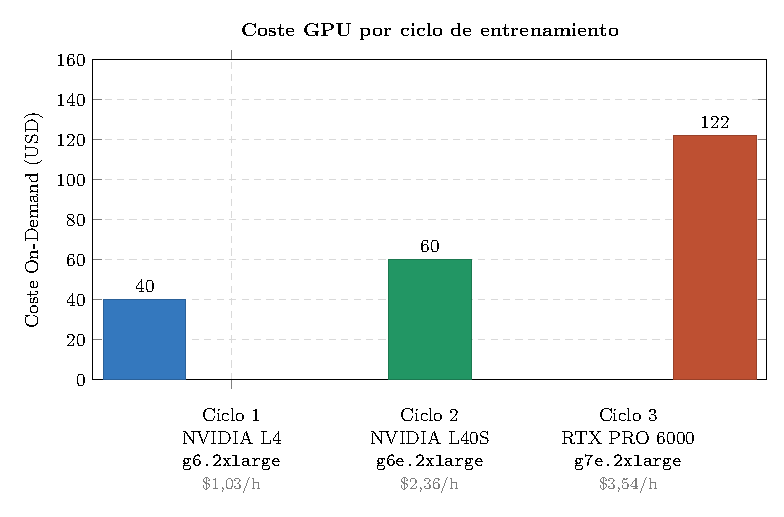
\includegraphics[width=0.72\textwidth]{images/diagrams_costes/cost_cycles_bar.pdf}
    \caption{Coste GPU por ciclo de entrenamiento. El incremento refleja la progresión hacia hardware más potente (mayor VRAM) necesaria para escalar el batch size y la estabilidad del entrenamiento.}
    \label{fig:cost_cycles}
\end{figure}

% ---------------------------------------------------------------
\subsection{Coste Humano: Ingeniero Junior en Data Science}

El coste más significativo de cualquier proyecto de desarrollo de software e IA no es el cómputo, sino el tiempo de las personas que lo desarrollan. Para contextualizar la inversión real del proyecto, se estima el coste equivalente de un \textbf{ingeniero junior en Data Science / Machine Learning} contratado en España.

\subsubsection{Referencia Salarial}

Según el mercado laboral español en 2025--2026, un perfil junior en Data Science con conocimientos de Python, PyTorch y cloud (AWS) presenta la siguiente horquilla retributiva:

\begin{table}[H]
\centering
\begin{tabularx}{\textwidth}{|X|c|c|}
\hline
\textbf{Concepto} & \textbf{Coste anual (EUR)} & \textbf{Coste mensual (EUR)} \\ \hline
Salario bruto anual (junior DS) & 25.000 & 2.083 \\ \hline
Seguridad Social a cargo empresa ($\approx$30\%) & 7.500 & 625 \\ \hline
\textbf{Coste total para la empresa} & \textbf{32.500} & \textbf{2.708} \\ \hline
\end{tabularx}
\caption{Coste empresarial estimado de un ingeniero junior en Data Science en España (2025--2026).}
\label{tab:coste_humano}
\end{table}

\subsubsection{Estimación para el Proyecto}

El proyecto se desarrolló durante \textbf{3 meses} a una dedicación de \textbf{4 horas diarias}, cubriendo el diseño de la arquitectura, la implementación del pipeline de datos, los tres ciclos de entrenamiento, la evaluación y la puesta en producción con infraestructura MLOps completa.

\begin{table}[H]
\centering
\begin{tabularx}{\textwidth}{|X|c|}
\hline
\textbf{Concepto} & \textbf{Valor} \\ \hline
Duración & 3 meses \\ \hline
Dedicación diaria & 4 h/día \\ \hline
Días laborables estimados & $\approx$66 días \\ \hline
\textbf{Horas totales trabajadas} & \textbf{$\approx$264 horas} \\ \hline
Coste hora empresa (32.500 EUR/año $\div$ 1.760 h/año) & 18,47 EUR/h \\ \hline
\textbf{Coste humano total} & \textbf{$\approx$4.876 EUR} \\ \hline
\end{tabularx}
\caption{Cálculo del coste humano a dedicación parcial (4h/día durante 3 meses).}
\label{tab:coste_horas}
\end{table}

\begin{table}[H]
\centering
\begin{tabularx}{\textwidth}{|X|c|c|}
\hline
\textbf{Concepto} & \textbf{Coste (EUR)} & \textbf{\%} \\ \hline
Coste humano (264h $\times$ 18,47 EUR/h) & $\approx$4.876 & 95,9\% \\ \hline
Infraestructura GPU (3 ciclos On-Demand) & $\approx$204 & 4,0\% \\ \hline
Almacenamiento y transferencia S3 & $<$5 & 0,1\% \\ \hline
\textbf{Coste total del proyecto} & $\approx$\textbf{5.085 EUR} & 100\% \\ \hline
\end{tabularx}
\caption{Coste total del proyecto combinando infraestructura y coste humano.}
\label{tab:coste_total}
\end{table}

\begin{figure}[H]
    \centering
    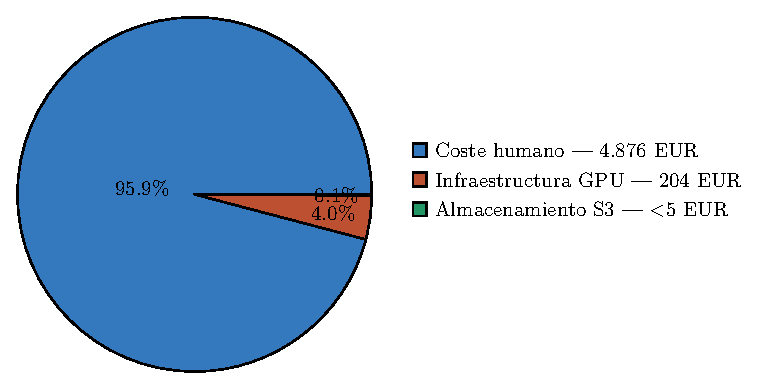
\includegraphics[width=0.65\textwidth]{images/diagrams_costes/cost_total_pie.pdf}
    \caption{Distribución porcentual del coste total del proyecto (5.085 EUR): el coste humano domina ampliamente con un 95,9\%, evidenciando que el cómputo cloud no es la barrera económica en proyectos de este tipo.}
    \label{fig:cost_total_pie}
\end{figure}

% ---------------------------------------------------------------
\subsection{Diagrama de Gantt}

La Figura~\ref{fig:gantt} muestra la distribución temporal de las tareas principales del proyecto a lo largo de las 12 semanas de desarrollo.

\begin{figure}[H]
    \centering
    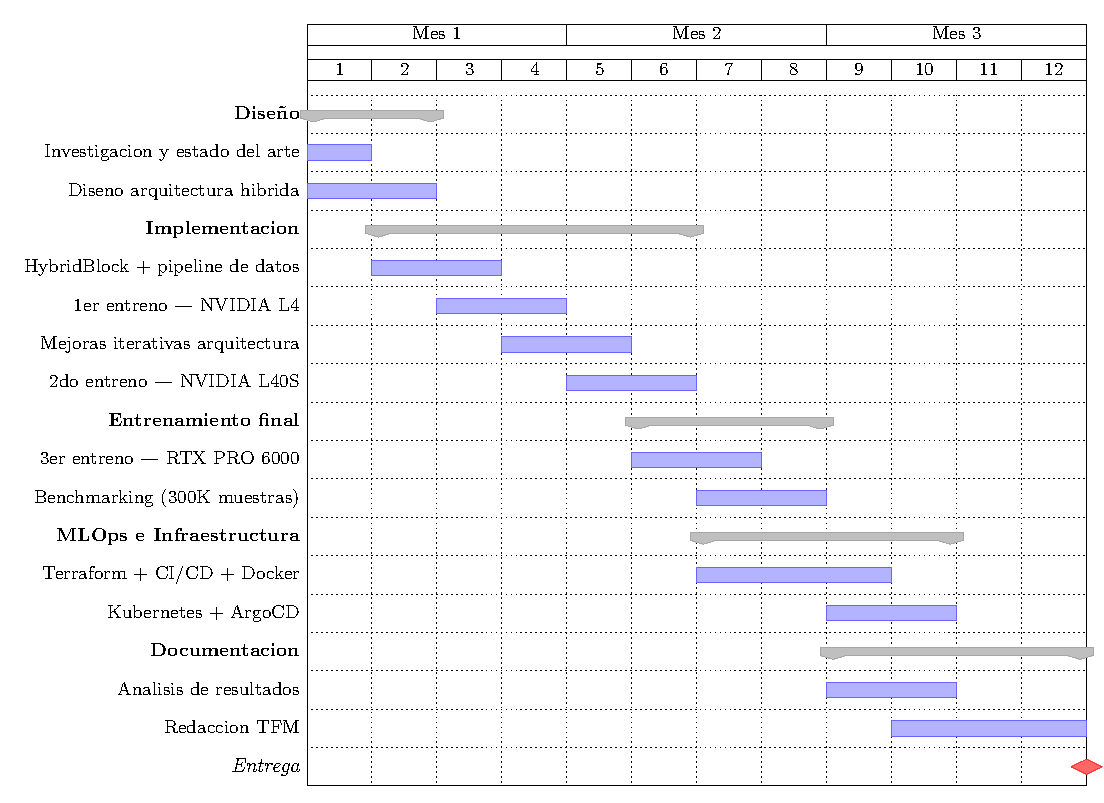
\includegraphics[width=\textwidth]{images/gantt_diagram/gantt.pdf}
    \caption{Diagrama de Gantt del proyecto (12 semanas, 4h/día). Cada unidad del eje horizontal representa una semana de trabajo.}
    \label{fig:gantt}
\end{figure}

% ---------------------------------------------------------------
\subsection{Análisis y Conclusiones de Costes}

La distribución de costes revela una conclusión importante: el coste de la infraestructura GPU representa únicamente el \textbf{4,0\%} del coste total del proyecto. El \textbf{95,9\% restante} corresponde al tiempo del ingeniero. Esta proporción es característica de proyectos de investigación aplicada donde el hardware cloud es accesible pero el capital humano cualificado es el recurso escaso.

\paragraph{Comparativa con alternativas.} Si se hubiera optado por fine-tuning de un modelo base (SmolLM2-135M, Phi-3-mini) en lugar de entrenamiento desde cero, el coste GPU se habría reducido a menos de \textbf{10 USD} (pocas horas de cómputo) mientras el coste humano habría permanecido igual. Esto refuerza la recomendación del Capítulo~\ref{sec:conclusiones}: en entornos con presupuesto restringido, optimizar el tiempo de ingeniería es más relevante que minimizar el gasto en cómputo.

\begin{figure}[H]
    \centering
    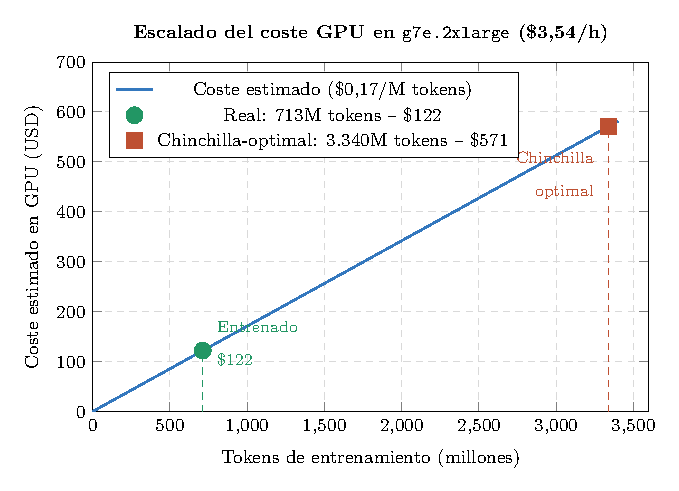
\includegraphics[width=0.85\textwidth]{images/diagrams_costes/cost_scaling.pdf}
    \caption{Escalado lineal del coste GPU en la instancia \texttt{g7e.2xlarge} (\$3,54/h). El punto verde marca el entrenamiento real (238M tokens, \$122); el punto rojo marca el umbral Chinchilla-optimal (3.340M tokens, \$1.716).}
    \label{fig:cost_scaling}
\end{figure}

\paragraph{Escalabilidad del coste GPU.} El ciclo de entrenamiento final (g7e.2xlarge, \$3,54/h) costó \$122 para procesar 713M tokens de entrenamiento (46.439 muestras $\times$ 1.024 $\times$ 15 épocas) en $\approx$34,5 horas. Alcanzar el volumen óptimo de Chinchilla~\cite{hoffmann2022chinchilla} (3.340M tokens, 4,7 veces el volumen actual) habría requerido $\approx$127 horas adicionales en la misma instancia, con un sobrecoste de $\approx$\textbf{\$449} y un \textbf{coste GPU total de $\approx$\$671} frente a los \$222 actuales. El coste total del proyecto con entrenamiento Chinchilla-optimal habría sido $\approx$\textbf{5.498 EUR} --- un incremento del 8,1\% respecto al actual. La barrera no es insuperable ni económica ni temporalmente, lo que refuerza que la decisión de usar más tokens era viable.
